%! program = pdflatex

\documentclass[letterpaper, 11pt]{article}
%\usepackage{geometry} 
%\geometry{letterpaper} 
\usepackage{graphicx}
\usepackage{amsmath}

\title{Regression Analysis of Life Cycle Cost Estimate}
\author{Michael Oexmann \& Steve Mazza}
\date{} 

\begin{document}

\maketitle
%\tableofcontents
\begin{abstract}
The task at hand is to try to find a Life Cycle Cost Estimate (LCCE) for a piece of commercial off-the-shelf (COTS) military equipment. We are given a sample of ten products with data corresponding to Operating Capacity, Horse Power, Weight, and Unit Price. We take the approach of creating a prediction model using regression analysis given the data from the sample provided.

We describe in detail the means by which we apply our analysis, using the statistical method of linear regression.  We state assumptions and limitations of the findings and discuss trade-offs driving the model selection.  We demonstrate and discuss the results of our analysis in detail.  Lastly, we draw conclusions supported by the results which include predictions as will as confidence intervals.
\end{abstract}

\section{Methodology}
Since our goal is to create a LCCE, we identify Unit Price as the response variable and Operating Capacity, Horse Power, and Weight were identified as potential predictors. We first utilize MiniTab to receive feedback on the data. We keyed in on two analysis tools, the Coefficient of Determination, $R^{2}$ and the $R^{2}$\emph{-adjusted}. The $R^{2}$ value measures how well future outcomes are likely to be predicted by the model. An $R^{2}$ value of 0 represent no correlation and an $R^{2}$ model of 1 represents perfect correlation. The $R^{2}$\emph{-adjusted} takes the analysis a step further by factoring in how well a predictor improves the model against what would be expected by chance.

Our key assumption is that the data is independent, unbiased, and accurately reflects the true population.  We base our findings on variations of a model of that determines Unit Price as a linear function of Operating Capacity, Horsepower, and Weight. \[ \mbox{Unit Price} \sim \mbox{Operating Capacity} + \mbox{Horsepower} + \mbox{Weight} \]
MiniTab optimizes for the highest $R^{2}$ value based on Multiple Linear Regression. This yields an equation using Operating Capacity, Horse Power, and Weight as predictors with an $R^{2}=67.3\%$ and $R^{2}\mbox{\emph{-adjusted}}=50.9\%$. Since MiniTab does not optimize for $R^{2}$\emph{-adjusted} we test the additional five combinations of predictors to try to find the highest $R^{2}$\emph{-adjusted}. This method would not be realistic in many large data sets with a high number of possible predictors, in those cases a heuristic would need to be utilized. Interestingly, we find that only using the predictors of Operating Capacity and Horse Power we are able to obtain a model with an $R^{2}=65.4\%$ and an $R^{2}\mbox{\emph{-adjusted}}=55.6\%$.

We continue further in our testing and model each individual predictor using a quadratic regression model and a cubic regression model. Our results netted only $R^{2}$ and $R^{2}$\emph{-adjusted} values that were smaller than we found using multiple linear regression models. Finally, we duplicate our results using the statistical packages in Excel and R. Since our results agree, we are confident and proceeded to look further at the output data.

\section{Analysis}
\subsection{Models}
We investigate two possible models. The requirements for the new equipment state an Operation Capacity of 5700, Horse Power of 83, and Weight of 1350. A risk associated with the stated requirements is that the Weight is outside of the range of the sample data. Thus the prediction is being extrapolated and must be considered as a potential technical issue. We further investigate the two models below.

\ \\
\textbf{Model 1: } \\
$\mbox{Unit Price} = 39367 + 6.85(\mbox{Operating Capacity}) \\
\mbox{\hspace{1.25cm}}- 215(\mbox{Horse Power}) + 0.87(\mbox{Weight})$ \\
$\$72312 = 39367 + 6.85 \times 5700 - 215 \times 83 + 0.87 \times 13500$ \\
$R^{2} = 67.3\%   R^{2}\mbox{\emph{-adjusted}} = 50.9\%$
\ \\ \ \\
\textbf{Model 2:} \\
$\mbox{Unit Price} = 35453 + 8.69(\mbox{Operating Capacity}) - 169(\mbox{Horse Power})$ \\
$\$70959 = 35453 + 8.69 \times 5700 - 169 \times 83$ \\
$R^{2} = 65.4\%   R^{2}\mbox{\emph{-adjusted}} = 55.6\%$ \\

The two yield similar results with \textbf{Model 1} resulting in an estimated cost of \$72312 vs. \$70959 for \textbf{Model 2}. The \$1353 difference represents a 1.9\% difference between the two. \\ \ \\ \ 
$\mbox{\textbf{Model 1:} Unit.Price} ~ \mbox{Operating Capacity} + \mbox{WT} + \mbox{HP}$ \\
$\mbox{\textbf{Model 2:} Unit.Price} ~ \mbox{Operating Capacity} + \mbox{HP}$ \\
\begin{center}
\begin{table}[htdp]
\caption{Comparison of Models}
\begin{center}
\begin{tabular}{lrrrrrr}
\hline
&  Res. Df &      RSS & Df  & Sum of Sq &     F & $Pr(>F)$  \\
\hline\hline
1  &    6 & 67296227 & & & & \\
2  &    7 & 71125661 & -1 &  -3829434 & 0.3414 & 0.5803  \\
\hline
\end{tabular}
\end{center}
\label{default}
\end{table}
\end{center}
\begin{center}
\begin{table}[htdp]
\caption{Analysis of Deviance}
\begin{center}
\begin{tabular}{lrrrrrr}
\hline
&  Step & Df & Deviance & Resid. Df & Resid. Dev &     AIC  \\
\hline\hline
1 & & &  &                       6 &  67296227 & 165.2203 \\
2 & - WT & 1 &  3829434      &   7 &  71125661 & 163.7737  \\
\hline
\end{tabular}
\end{center}
\label{default}
\end{table}
\end{center}
An aspect of both equations that we find interesting is that Horse Power has a negative result on the Unit Cost. Logically higher Horse Power would result in a higher price but as sometimes found in regression models, prediction models do not always follow what would logically be expected.

\subsection{Raw Data}
The following table summarizes the raw data, providing a quick glance at the values before fitting with our model.
\begin{center}
\begin{table}[htdp]
\caption{Summary Statistics}
\begin{center}
\begin{tabular}{rlrlrlrl}
\hline
\multicolumn{2}{c}{Operating Capacity} & \multicolumn{2}{c}{Horsepower}  & \multicolumn{2}{c}{Weight} & \multicolumn{2}{c}{Price}  \\
\hline\hline
Min.: & 5000 & Min.: & 54.0 & Min.: & 10000 & Min.: & 60560 \\
1st Qu.: & 5500 & 1st Qu.: & 64.0 & 1st Qu.: & 10072 &  1st Qu.: & 68690 \\
Median: & 5500 & Median: & 82.0 & Median: & 10823 & Median: & 70845 \\
Mean: & 5550 & Mean: & 77.8 & Mean: & 11404 & Mean: & 70575 \\
3rd Qu.: & 5875 & 3rd Qu.: & 84.0 & 3rd Qu.: & 12861 & 3rd Qu.: & 72490 \\
Max.: & 6000 & Max.: & 101.0 & Max.: & 13496 & Max.: & 78870  \\
\hline
\end{tabular}
\end{center}
\label{default}
\end{table}
\end{center}

\subsection{Fit Data}
The following three tables provide different summary views into the results of our regression model with optimization for $R^{2}$.
\begin{center}
\begin{table}[htdp]
\caption{Residuals}
\begin{center}
\begin{tabular}{rrrrr}
\hline
Min & 1Q & Median & 3Q & Max  \\
\hline\hline
-5178.6 & -1165.3 &  -343.6 &  1529.7 &  4379.8 \\
\hline
\end{tabular}
\end{center}
\label{default}
\end{table}

\begin{table}[htdp]
\caption{Coefficients}
\begin{center}
\begin{tabular}{lrrrr}
\hline
& (Intercept) & Operating Capacity   &      WT    &       HP  \\
\hline\hline
1 &  -5503.17792  &        0.9840296 &  0.37278491 & -58.46027443 \\
2  &  2948.99739  &       -0.3928200 & -0.10282755 &   2.99389462 \\
3  &   510.92709   &      -0.3468143 &  0.12830423 &   0.23114019 \\
4 &   -170.65700   &      -0.5898346 &  0.27883642 &   0.18324120 \\
5 &    330.69285   &       0.5378408 & -0.25097123 &  -2.64041020 \\
6 &  -9243.33311    &      0.7012806 &  0.81803718 & -42.56878211 \\
7 &  15255.11204   &      -3.1101710 &  0.25227829 &  -20.35803405 \\
8 &   -2261.44385    &      1.2292114 & -0.69945008 &  49.46004333 \\
9 &  -31071.66683   &       7.0713242 &  -1.94222948 & 169.94221871 \\
10 &    46.28448  &        0.1599711 & -0.07562419 &  -0.04969748 \\
\hline
\end{tabular}
\end{center}
\label{default}
\end{table}

\begin{table}[htdp]
\caption{Coefficient Summary}
\begin{center}
\begin{tabular}{lrrrr}
\hline
& Estimate & Std. Error & $t$-value & $Pr(>\mid t\mid)$  \\
\hline\hline
(Intercept) & 39366.9207 & 18341.2672 & 2.146 & 0.0755 \\
Operating Capacity & 6.8496 & 4.3968 & 1.558 & 0.1703  \\
Weight & 0.8667 & 1.4832 & 0.584 & 0.5803  \\
Horsepower & -214.5313 &105.4082 & -2.035 & 0.0880 \\
\hline
\end{tabular}
\end{center}
\label{default}
\end{table}
\end{center}
Residual standard error: 3349 on 6 degrees of freedom \\
Multiple $R^{2}$: 0.6729,	Adjusted $R^{2}$: 0.5094 \\
$F$-statistic: 4.115 on 3 and 6 DF,  $p$-value: 0.06643 

\begin{center}
\begin{table}[htdp]
\caption{ANOVA}
\begin{center}
\begin{tabular}{lrrrrr}
\hline
& DoF &   Sum Sq & Mean Sq & $F$-value & $Pr(>\mid t\mid)$  \\
\hline\hline
Operating Capacity &  1 & 70344680 & 70344680 &  6.2718 & 0.04625 \\
WT &                 1 & 21657329 & 21657329 & 1.9309 & 0.21403  \\
HP &                  1 & 46459179 & 46459179 & 4.1422 & 0.08802 \\
Residuals &           6 & 67296227 & 11216038 & & \\
\hline
\end{tabular}
\end{center}
\label{default}
\end{table}
\end{center}
Signif. codes:  0 �***� 0.001 �**� 0.01 �*� 0.05 �.� 0.1 � � 1

\begin{center}
\begin{table}[htdp]
\caption{Confidence/Prediction Intervals}
\begin{center}
\begin{tabular}{lrrrr}
\hline
Obs &   Fit & SE Fit   &   95\% CI     &     95\% PI  \\
\hline\hline
  1 &  62048  &  2555 & (56006, 68090) & (52388, 71708) \\
  2 &  73441  &  1656 & (69525, 77357) & (64947, 81935) \\
  3 & 66226  &  1878 & (61784, 70668) & (57477, 74975) \\
  4 & 72469  &  1361 & (69250, 75688) & (64273, 80665) \\
  5 & 72638  &  1407 & (69311, 75964) & (64399, 80877) \\
  6 & 73947  &  1642 & (70065, 77830) & (65469, 82426) \\
  7 & 73610  &  1649 & (69712, 77508) & (65124, 82096) \\
  8 & 69094  &  1108 & (66473, 71716) & (61114, 77075) \\
  9 & 69810  &  2314 & (64338, 75281) & (60495, 79124) \\
 10 & 72469 &   1361 & (69250, 75688) & (64273, 80665) \\
\hline
\end{tabular}
\end{center}
\label{default}
\end{table}
\end{center}

\begin{center}
\begin{table}[htdp]
\caption{Confidence Interval Summary}
\begin{center}
\begin{tabular}{lrr}
\hline
& 2.5 \%  &  97.5 \%  \\
\hline\hline
(Intercept)  &      -5512.543325 & 84246.38475 \\
Operating Capacity  &  -3.908919  &  17.60818 \\
WT        &            -2.762580  &   4.49588 \\
HP           &       -472.455924  &  43.39340 \\
\hline
\end{tabular}
\end{center}
\label{default}
\end{table}
\end{center}

\begin{center}
\begin{table}[htdp]
\caption{Predictions}
\begin{center}
\begin{tabular}{rrr}
\hline
       fit  &    lwr  &    upr  \\
\hline\hline
       72303.49 & 66123.85 & 78483.14 \\
\hline
\end{tabular}
\end{center}
\label{default}
\end{table}
\end{center}

\subsection{Graphical Analysis}
The Residual Plots seem to have a more or less horizontal appearance, indicating that using a linear regression test model is a fairly accurate representation of the data. As well, the width and distribution along the x-axis is mostly uniform, indicating an unbiased model. The residuals look sufficiently distributed such that a large $R^{2}$ value, $R^{2} > 80\%$, may be difficult to achieve. Observation 7 has the largest residual value and should be monitored as a potential outlier but is not so rare to warrant great concern.

The Cumulative Distribution Function (CDF) depicts the fit equation for $R^{2}$ and its 95\% Confidence Interval of unit cost. This shows graphically thresholds within which we are 95\% confident that the true mean unit cost for the given parameters will be captured. 
\begin{center}
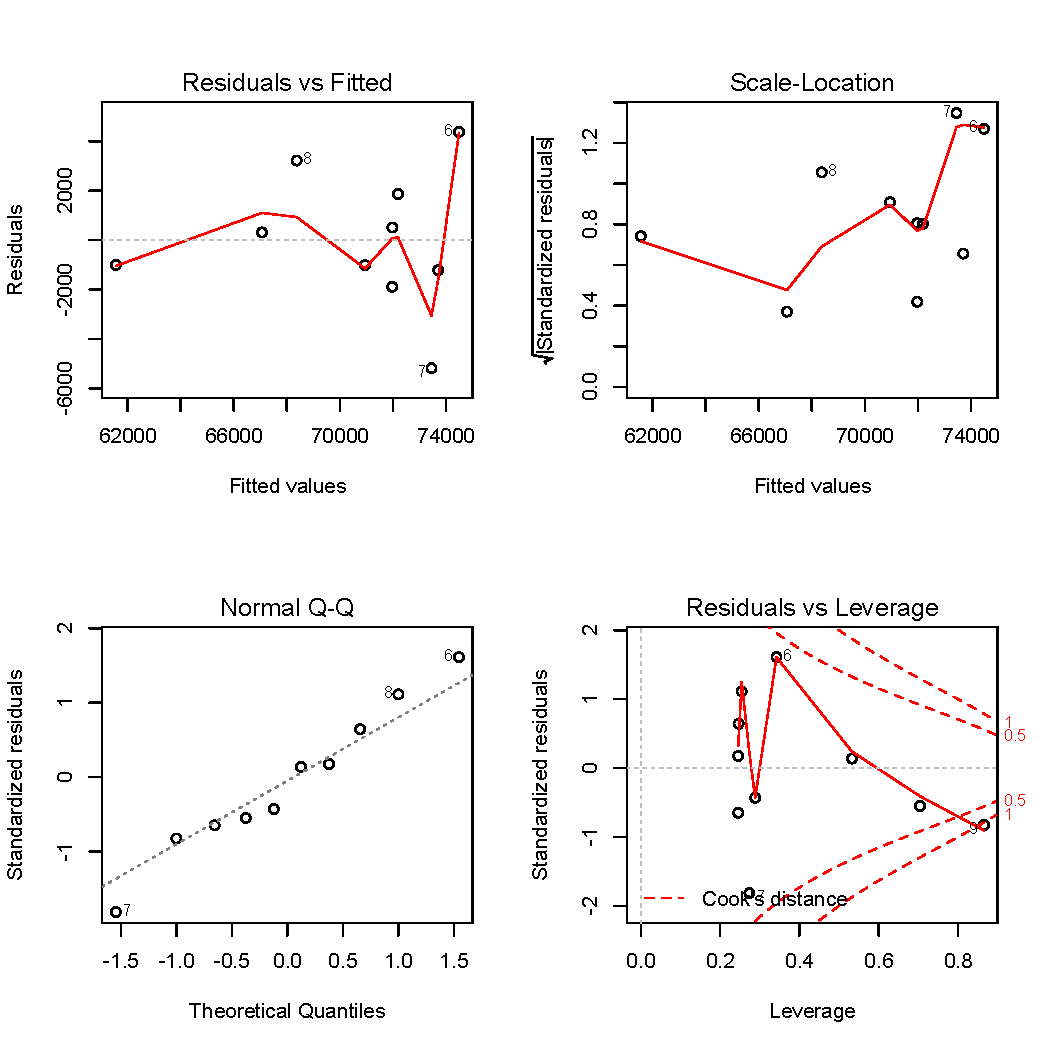
\includegraphics[scale=0.75]{Rplot.pdf}
\end{center}
\begin{center}
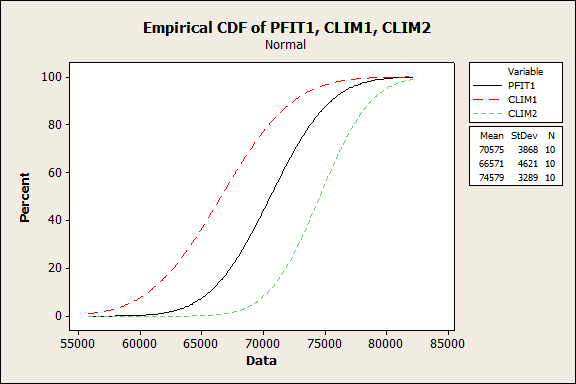
\includegraphics[scale=0.5]{ecdf.jpg}
\end{center}

\section{Conclusion}
We draw conclusions supported by the Results (above). These include predictions as will as confidence intervals. 

Analysis of the data presented suggests that the point estimate of the cost of the new equipment based on $\mbox{Unit Cost} = 39367 + (6.85 \times\mbox{Operating Capacity}) - (215\times\mbox{Horse Power}) + (0.87\times\mbox{Weight})$ with requirements of 5700 Operating Capacity, 83 Horse Power, and 13500 lbs is a Unit Cost of 72303.49. Although this model did not have the highest $R^{2}$\emph{-adjusted} it did have the highest value for the commonly utilized $R^{2}$. This model also was chosen had the more conservative price estimate using a 95\% confidence interval which yields a lower bound of 66123.85 and an upper bound of 78483.14 to quantify uncertainty.

\end{document}